\documentclass[journal]{IEEEtran}

\usepackage{amsmath,amssymb}
\usepackage{booktabs}
\usepackage{graphicx}
\usepackage{placeins}
\usepackage{tabularx}
\usepackage{xurl}
\usepackage[hidelinks]{hyperref}

\usepackage{iftex}
\ifXeTeX
  \makeatletter
  \@ifpackageloaded{fontspec}{}{\usepackage{fontspec}}
  \makeatother
  \usepackage{xeCJK}
  \xeCJKsetup{CJKspace=true}
  \defaultfontfeatures{Ligatures=TeX}
  \IfFontExistsTF{TeX Gyre Termes}{%
    \setmainfont{TeX Gyre Termes}%
  }{%
    \IfFontExistsTF{Times New Roman}{%
      \setmainfont{Times New Roman}%
    }{%
      \setmainfont{STIX Two Text}%
    }%
  }
  \IfFontExistsTF{NanumBarunGothicOTF}{%
    \setCJKmainfont[
      ItalicFont={NanumBarunGothicOTF},
      SmallCapsFont={NanumBarunGothicOTF}
    ]{NanumBarunGothicOTF}%
    \setCJKsansfont{NanumBarunGothicOTF}%
    \setCJKmonofont{NanumBarunGothicOTF}%
  }{%
    \IfFontExistsTF{Noto Sans CJK KR}{%
      \setCJKmainfont[
        ItalicFont={Noto Sans CJK KR},
        SmallCapsFont={Noto Sans CJK KR}
      ]{Noto Sans CJK KR}%
      \setCJKsansfont{Noto Sans CJK KR}%
      \setCJKmonofont{Noto Sans CJK KR}%
    }{%
      \setCJKmainfont[
        Scale=0.92,
        ItalicFont={Apple SD Gothic Neo},
        SmallCapsFont={Apple SD Gothic Neo}
      ]{Apple SD Gothic Neo}%
      \setCJKsansfont[Scale=0.92]{Apple SD Gothic Neo}%
      \setCJKmonofont[Scale=0.92]{Apple SD Gothic Neo}%
    }%
  }
  \xeCJKDeclareCharClass{Default}{"00B7}
\else
  \usepackage{kotex}
\fi

\newif\ifanonymoussubmission
\ifdefined\ANONBUILD
  \anonymoussubmissiontrue
\else
  \anonymoussubmissionfalse
\fi

\newcommand{\system}{TRACE-RPG}
\newcommand{\Valid}{\mathrm{valid}}
\newcommand{\AcceptSet}{\mathcal{A}}
\newcommand{\GoalSet}{\mathcal{G}}
\newcommand{\HitSet}{\mathcal{H}}
\newcommand{\SchemaSet}{\mathcal{S}}
\newcommand{\RepoURL}{\ifanonymoussubmission [Anonymous Repository URL withheld for double-anonymous review]\else \url{https://github.com/akillness/neural_symbolic_in_game}\fi}
\AtBeginDocument{\emergencystretch=2.5em}
\providecommand{\Description}[2][]{}

\anonymoussubmissionfalse

\setlength{\tabcolsep}{4pt}
\renewcommand{\arraystretch}{1.02}
\AtBeginDocument{%
  \setcounter{dbltopnumber}{1}%
  \renewcommand{\topfraction}{0.92}%
  \renewcommand{\dbltopfraction}{0.92}%
  \renewcommand{\textfraction}{0.05}%
  \renewcommand{\floatpagefraction}{0.88}%
  \renewcommand{\dblfloatpagefraction}{0.88}%
}

\title{TRACE-RPG: 에이전트 게임 시스템을 위한 감사 가능한 엔진 제안--커밋 경계와 온톨로지 검증}

\author{정장영$^{1}$, 강신진$^{2,*}$\\
\small $^{1}$홍익대학교 게임학과 (제1저자)\\
\small $^{2}$홍익대학교 교수 (교신저자)\\
\small $^{*}$교신저자}

\begin{document}
\maketitle

\begin{abstract}
스키마에 부합하는 게임 내 행동 제안이라도 접근 불가 물체 요구, 비인가 상태 전이, 조기 비밀 공개를 포함할 수 있다. 플레이어 경험·인간 평가는 후속 과제($N{=}0$)로 명시 분리하고 게임 엔진 런타임 안전성과 결정론적 재현성에 초점을 맞추어, \system{}는 \texttt{nesy\_game.multihop}의 이행적 Datalog 폐쇄, 7술어 게이트, 상태 비참조 수리 $\rho(a,E)$, 해시 연쇄 리플레이로 제안·커밋 권한을 분리한다(정리 1--4, \textbf{I1--I4}). 1,664건 유한 그래프 감사, Godot~4.7.1 장기 실행(1,600틱, p95 0.708\,ms), 480건 $R{\le}64, d{\le}5$ Datalog 검증(100.0\%, $\le$7.12\,$\mu$s)에 이어, 직접 HTTPS Anthropic Claude~5.5 API(Haiku·Sonnet·Opus~5.5, deprecated \texttt{temperature} 생략·\texttt{output\_config.json\_schema}) 및 3모델군 CLI 평가는 다음을 보인다: 105회 독립 5턴 폐루프(\textbf{P15}: 15/15 무누출·0 위험, 정리~2 $\rho_{\mathrm{repairs}}{=}0$ 무세탁 실증·하이브리드 \textbf{15/15} 목표 대 Safe-RL 0/15·NeMo 1/15), 60회 요인 실험(\textbf{P16A}: \texttt{ontology\_multihop} 30/30·22건 $\rho$수리·11/30 대 규칙 22/30·0/30), Godot~4.7.1 인증 21회+CLI 42회(\textbf{P16B}, \textbf{P13}: 전량 리플레이 일치, 제품 6/6 해시 일치, 0/63 누출), $(a,E)$ 동등 수리 27/27(0토큰), 통합 540회 한·영 우회(\textbf{P17}: $\kappa{=}0.8813$, 0\% FRR), Croissant~1.0 v5(26/26), 격리된 \texttt{TR01--TR06}($N{=}0$).
\end{abstract}

\begin{IEEEkeywords}
게임 엔진 검증, 뉴로심볼릭 시스템, 액션 실딩, 반례 수리, 결정론적 리플레이
\end{IEEEkeywords}

\section{서론}
스키마에 부합하는 게임 내 행동 제안이라도 접근할 수 없는 물체를 요구하거나 권한이 없는 상태 전이, 혹은 현재 시점에서 공개할 수 없는 비밀 발화를 포함할 수 있다. 서사적 정합성(grounding)과 개연성 있는 대화 생성 \cite{S03_weir2024ontologically,S20_ashby2023personalized}은 후보 콘텐츠를 제공할 뿐이며, 게임 엔진은 현재 상태에서 어떤 전이를 승인할지 별도로 판정해야 한다.

\system{}는 이 판정을 외부의 제안--커밋(proposal-to-commit) 경계에서 강제한다(그림~\ref{fig:architecture}). 모델과 어댑터가 구조화된 후보를 제출하면 결정론적 게이트가 행동 정책, 선행조건, 물체 도달 가능성, NPC 지식, 정보 공개 권한, 효과, 퀘스트 단계 단조성을 검사한다. 검사에 실패하면 게이트는 제한된 수리를 위한 구조화된 오류를 반환하며, 수리는 정본 상태(canonical state)가 아닌 후보만 수정하고 동일 상태 재검증을 통과한 경우에만 상태를 갱신한다. 여덟 역할 읽기 전용 온톨로지 뷰는 쓰기 권한 없이 출처 선언과 검사·결정을 연결하며, 해시 연결 전이 기록은 의미적 리플레이와 배정 전수 회계(assignment-complete accounting)를 보장한다.

개념적으로 이 계약은 단순 사실 일치(factual grounding)를 넘어 NPC의 \emph{인식론적 지식 경계}(행위자가 알고 있는 사실)와 \emph{정보 공개 권한 정책}(현재 퀘스트 단계에서 발화할 수 있는 사실)을 분리한다. 방법론적으로는 LLM 호출이 0회인 결정론적 검증 계층(게이트 검사, 유도 수리, 엔진 리플레이)과 실패를 누락 없이 보존하는 제한된 확률적 제안기 계층을 엄격히 분리한다.

결정론적 감사에서 스키마 전용 대조군은 32개 유한 그래프 조합에서 무효 제안 260/416건을 커밋한 반면 의미 게이트는 \textbf{0/416} 위험 커밋·0/156 오거부·128/260건 $\rho$ 수리를 기록했고, $R{\le}64, d{\le}5$ 480건 Datalog 검증(\textbf{P9})에서 \texttt{nesy\_game.multihop}만이 $\le$7.12\,$\mu$s로 100.0\% 정확도를 달성하였다($Q{=}1100.19$). 정리 1--4(\textbf{I1--I4})를 토대로, Haiku·Sonnet·Opus~5.5 직접 HTTPS Anthropic API 평가는 105회 독립 5턴 폐루프 협상(\textbf{P15}: 15/15 무누출·0 위험·하이브리드 15/15 목표 대 Safe-RL~\cite{alshiekh2018shield} 1/15·NeMo 스타일~\cite{rebedea2023nemo} 1/15), 60회 요인 실험(\textbf{P16A}: \texttt{ontology\_multihop} 30/30 무누출·22건 수리 대 22/30 \texttt{general\_rule}), 21회 Godot~4.7.1 폐루프(\textbf{P16B}: 21/21 재실행 일치, 제품 6/6 해시 일치), 540회 통합 한·영 우회(\textbf{P17}: $\kappa{=}0.8813$, 0\% FRR)를 입증하며, 3모델군 CLI(\textbf{P11}--\textbf{P14}: $(a,E)$ 수리 27/27 0토큰), \texttt{DATASHEET\_v5.md}~\cite{gebru2021datasheets}, Croissant~1.0 v5~\cite{akhtar2024croissant}(26/26), 격리된 \texttt{TR01--TR06}($N{=}0$, \texttt{AWAITING\_HUMAN\_RATERS})으로 공개 경계를 완결한다.

\section{관련 연구와 연구 공백}
정합성, 기억, 계획, 역할 기반 에이전트 \cite{S03_weir2024ontologically,S20_ashby2023personalized,S07_park2023generative,S08_shao2023character} 및 플레이어·대화 시스템 \cite{S21_akoury2023player,S22_hochreiter2026beyond,S23_yin2026contextualized,S02_figueiredo2025scaffolded}은 맥락적 상호작용을 지원하는 반면, 본 연구는 인코딩된 현재 상태와 공개 정책이 제안된 전이를 허용하는지를 판정한다. 정서 및 몰입 모델링 \cite{S24_yannakakis2011experiencedriven,S25_melhart2020engagement,S26_wang2026engagement}은 생성 스타일을 안내할 뿐 상태 변경 권한을 부여하지 않는다.

기존 벤치마크와 자동 플레이테스팅은 상태, 체화 환경, 콘텐츠, 과정, 사회적 상호작용, 장기 과업을 다루며 \cite{S11_cote2019textworld,S12_wang2022scienceworld,S13_fan2022minedojo,S14_perezliebana2019gvgai,S15_liu2024agentbench,S16_ma2024agentboard,S17_zhou2024sotopia,S18_paglieri2025balrog,S19_lepelletier2022playtesting}, NCP-Bench는 서사적 일관성과 사실 정합성을 평가한다 \cite{S58_ma2026ncpbench}. 문법·스키마·어포던스·안전 실딩 기법 \cite{S09_geng2023grammar,S10_beurerkellner2023prompting,S36_scholak2021picard,S50_kambhampati2024llmmodulo,S51_ichter2023saycan,S52_wang2025agentspec,S53_li2025settingdc,S54_zhou2025story2game,S42_buongiorno2024pangea,alshiekh2018shield,rebedea2023nemo}, 반례 기반 수리 \cite{S45_madaan2023selfrefine,S48_shinn2023reflexion,S46_chen2023selfdebug,S47_solarlezama2006sketching}, 재현성·데이터셋 표준 \cite{S31_agarwal2021precipice,S33_pineau2021reproducibility,S56_feng2025agentrr,S59_sun2025bdc,gebru2021datasheets,akhtar2024croissant}이 본 설계의 토대다. 스키마 적합성과 행위 합법성, 또는 사실 정합성과 발화 안전성을 동일시하던 선행 연구와 달리, \system{}는 스키마 파싱, 인식론적 지식, 공개 권한, 정본 상태 커밋을 독립 감사 가능한 게이트로 분리한다.


\begin{figure*}[!t]
  \centering
  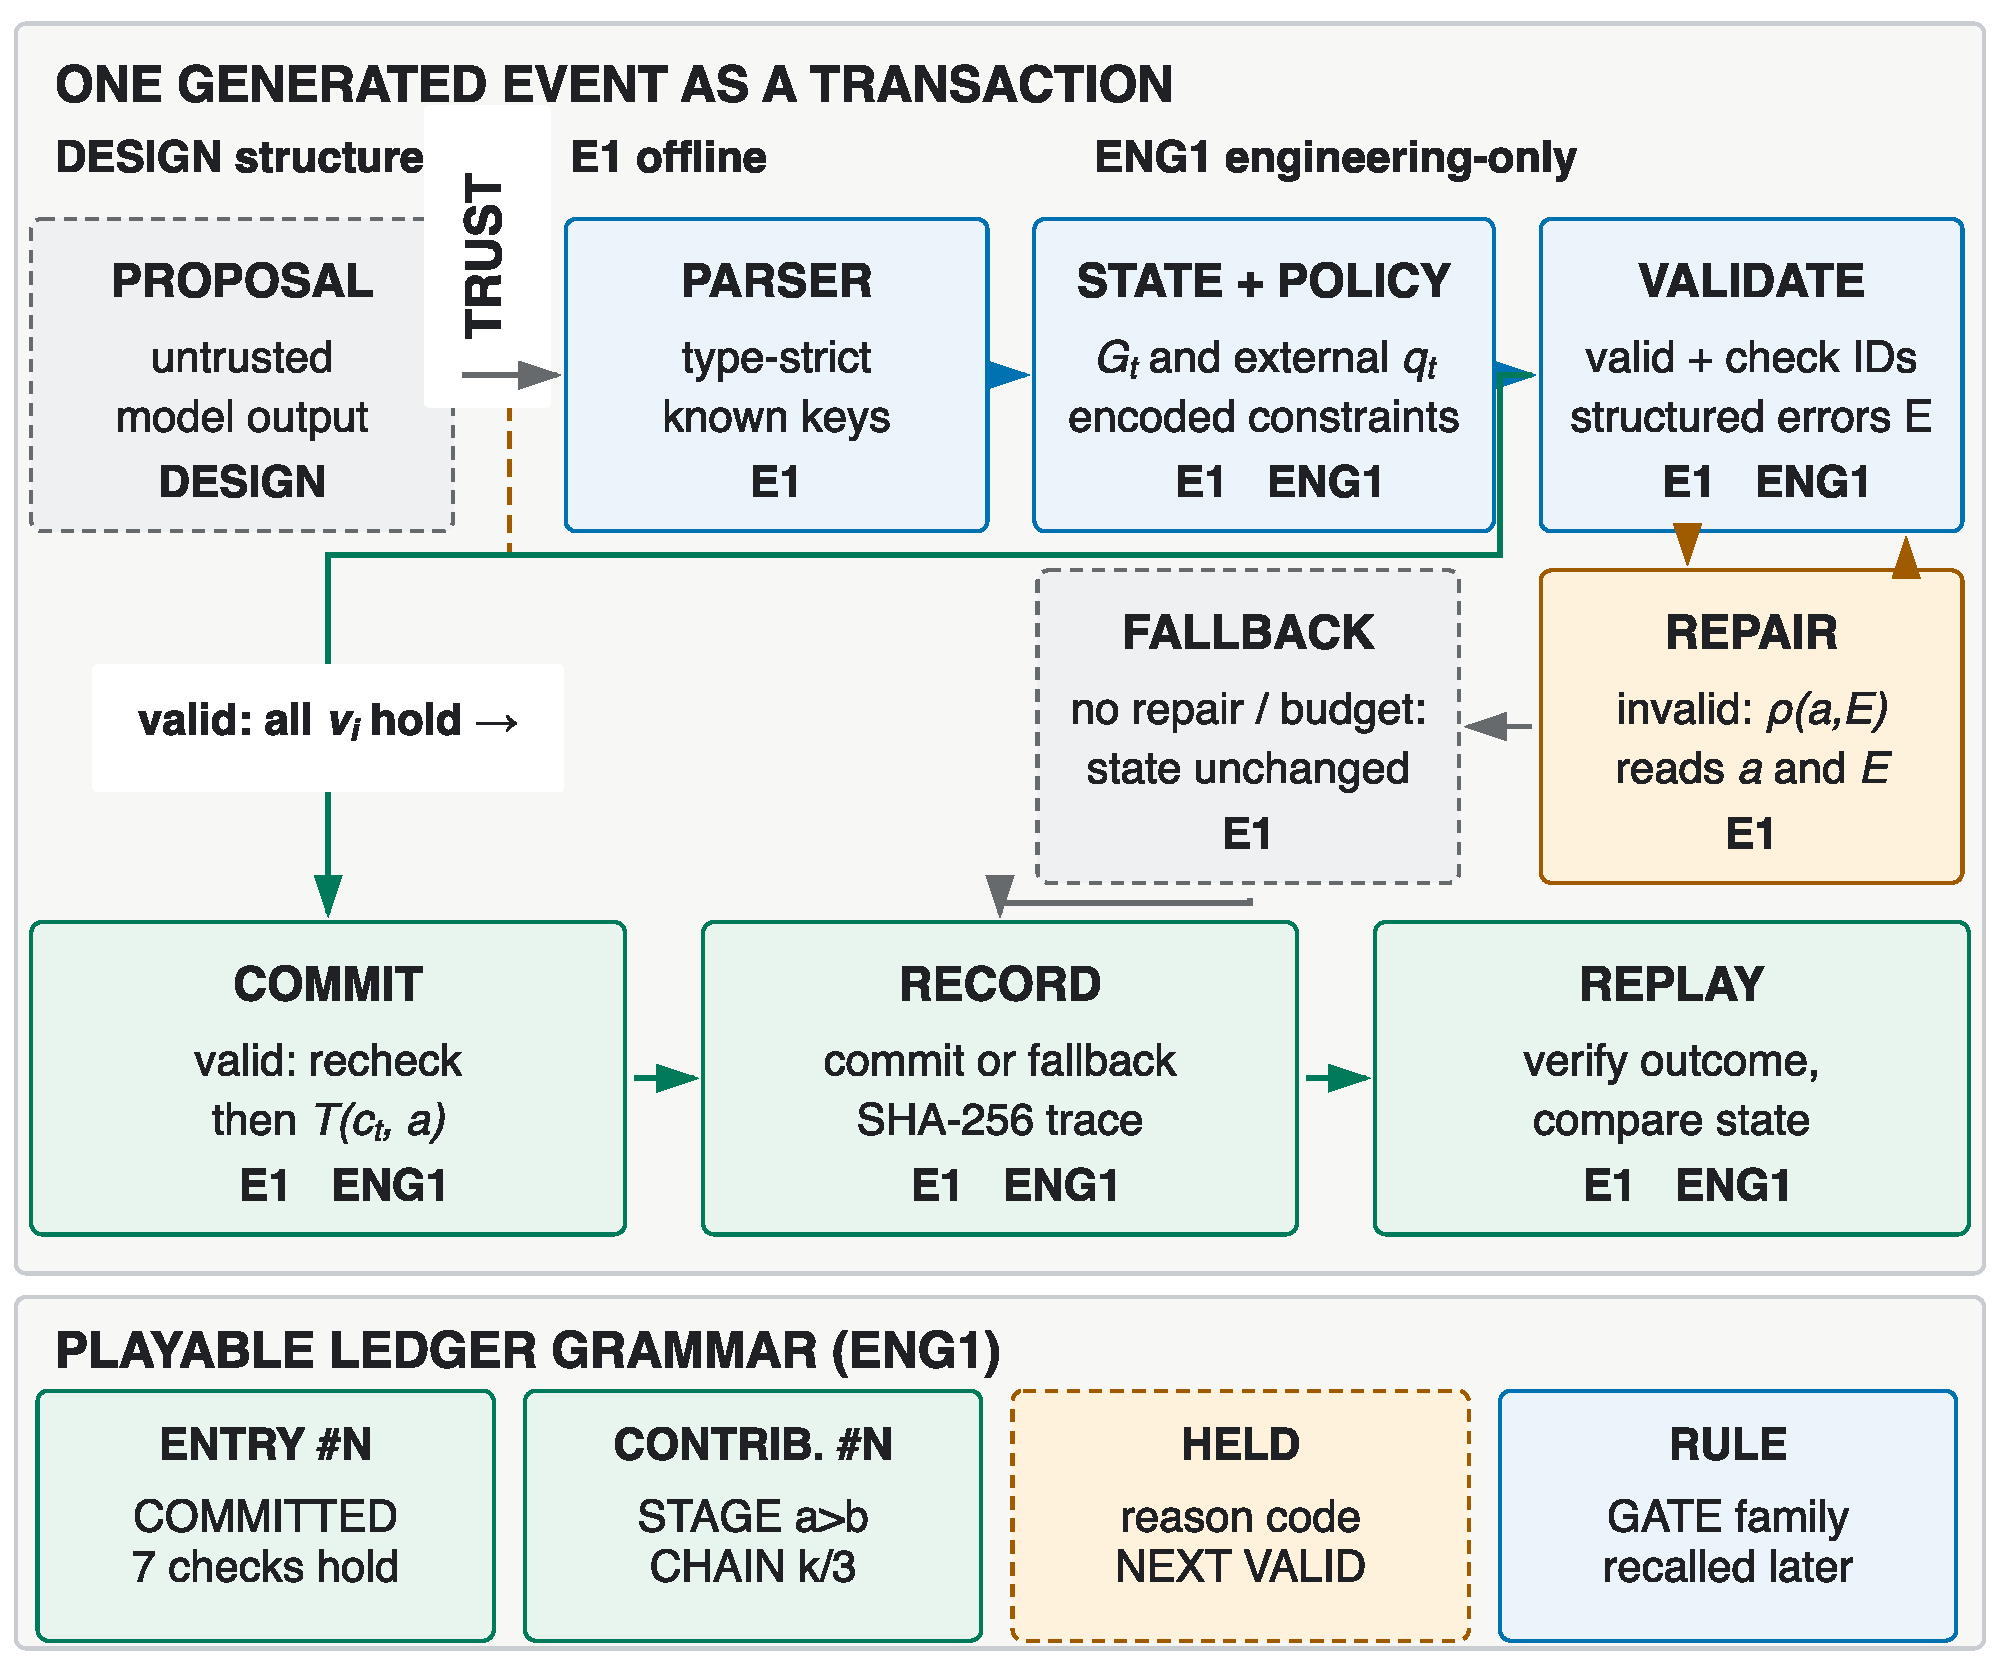
\includegraphics[width=0.64\textwidth]{../../figures/fig_architecture.pdf}
  \caption{정책과 상태 $c_t$가 제안을 게이팅한다. 오류는 제한된 $\rho$ 수리 또는 상태 불변 fallback으로 이어지며, 통과 후보는 재검증 뒤 커밋·기록·리플레이된다.}
  \label{fig:architecture}
\end{figure*}

\section{문제 정의와 보장 경계}\label{sec:problem}
입력 $c_t=(G_t,q_t)$에서 $G_t$는 형식이 지정된 게임 스냅샷(장소, 도달 가능 위치, 물체 배치, 소지품, 사실, NPC 지식, 퀘스트 단계)을, $q_t$는 외부에서 저작된 행동 정책·정보 공개·퀘스트 단계 제약을 나타낸다. 검증 술어는 직전 이력 $h_{<t}$를 역산하거나 $q_t$를 변경하지 않으며, 검색 결과나 정서 점수는 쓰기 권한이 없다.

비신뢰 제안 $a_t$를 엄격히 파싱한 뒤, 검증기는 7개의 결정론적 술어를 실행하여 \texttt{ValidationResult}(\allowbreak$\mathrm{valid},E_t,C_{\mathrm{run}}$)를 반환한다:
\begin{equation}
\begin{aligned}
V(c_t,a_t)&=(\mathrm{valid},E_t,C_{\mathrm{run}}),\\
\boldsymbol{v}&=(v_{\mathrm{policy}},v_{\mathrm{pre}},v_{\mathrm{reach}},\\
&\qquad v_{\mathrm{know}},v_{\mathrm{disc}},v_{\mathrm{elig}},v_{\mathrm{stage}})\in\{0,1\}^{7},
\end{aligned}
\end{equation}
여기서 $\mathrm{valid}\equiv\bigwedge_{i=1}^{7}(v_i=1)$이며, $E_t$는 오류 코드·개체·원인·수리 힌트를 기록한다. 정본 상태는 7개 술어를 모두 통과한 경우에만 갱신된다:
\begin{equation}
c_{t+1}=\begin{cases}
T(c_t,a_t), & \bigwedge_{i=1}^{7}(v_i=1),\\
c_t, & \text{otherwise.}
\end{cases}
\label{eq:transition}
\end{equation}

\subsection{스키마 유효성, 권한, 목표 달성의 분리}\label{sec:authorization-sets}
행동 전 상태 $c_t$, 저작 정책, 엄격 스키마를 고정하고 스키마 유효 후보 집합을 $\SchemaSet$라 할 때, 권한과 목표 달성을 다음과 같이 분리한다:
\begin{equation}
\begin{aligned}
\AcceptSet(c_t)&=\{a\in\SchemaSet:V(c_t,a).\mathrm{valid}\},\\
\GoalSet(c_t)&=\{a\in\SchemaSet:\operatorname{Goal}(T(c_t,a))\},\\
\HitSet(c_t)&=\AcceptSet(c_t)\cap\GoalSet(c_t)\subseteq\AcceptSet(c_t)\subseteq\SchemaSet.
\end{aligned}
\end{equation}
금지 사실을 선언한 스키마 유효 후보는 $\AcceptSet$ 밖에 놓이며, 허용된 관찰 행동은 $\AcceptSet$에 속하지만 $\GoalSet$ 밖에 놓일 수 있다. 지식과 공개 권한은 독립 입력이다. 예컨대 NPC는 0단계와 1단계 모두에서 \texttt{keeper\_\allowbreak secret}을 알고 있으나, 공개는 0단계에서 금지되고 1단계에서 허용된다.

\subsection{불변식 I1--I4에 대한 형식 안전성 정리}\label{sec:formal-proofs}
결정론적 전이 규칙(식~\eqref{eq:transition})과 엄격 파서 \texttt{parse\_}\allowbreak\texttt{candidate\_}\allowbreak\texttt{mapping} 아래에서 불변식 \textbf{I1--I4}는 임의의 유한 인코딩 상태 $c_t=(G_t,q_t)$, 수리 예산 $K\in\mathbb{Z}_{\geq 0}$ 및 정상 반환 콜백에 대한 조건부 구조 정리로 성립한다.

\noindent\textbf{정리 1 (I1: 상태 보존 안전성).} \emph{초기 후보가 엄격 파싱을 통과하지 못하거나 $K{+}1$회 모든 시도에서 $V(c_t,a^{(j)}).\mathrm{valid}=\mathrm{false}$이면 $c_{t+1}=c_t$이며 커밋된 효과는 비어 있다.}
\par\noindent\textit{증명.} \texttt{parse\_}\allowbreak\texttt{candidate\_}\allowbreak\texttt{mapping}은 커밋 전에 비정형 제안을 거부하며, 그림~\ref{alg:commit}에서 $\operatorname{Commit}$은 $\mathrm{ok}=\mathrm{true}$일 때만 도달 가능하고 $j=K$에서는 $\operatorname{Fallback}(c_t)$이 식~\eqref{eq:transition}에 의해 $c_t$를 그대로 반환한다. \hfill$\square$

\noindent\textbf{정리 2 (I2: 유한 종료와 상태 비참조 세탁 방지 수리).} \emph{유한 $K{\geq}0$과 정상 반환 콜백 하에서 루프는 $V$를 최대 $K{+}1$회 호출하며, 상태 변경 직전 $V(c_t,a^{(j)})$를 재검증하고, $\rho$는 \texttt{WorldState} 의존 권한 오류 클래스를 변경하지 않는다.}
{\sloppy\par\noindent\textit{증명.} 계수기 $j$는 $0$에서 시작하여 증가 전 $j=K$를 검사하므로 $V$ 호출은 최대 $K{+}1$회로 유계다. 표~\ref{tab:rho-rules}에 따라 $\rho(a,E)$는 \texttt{WorldState}를 읽지 않고 $(a,E)$만 입력받아 \texttt{UNKNOWN\_}\allowbreak\texttt{ACTION\_}\allowbreak\texttt{TYPE}, \texttt{UNREACHABLE\_}\allowbreak\texttt{REQUIRED\_}\allowbreak\texttt{OBJECT}, \texttt{NPC\_}\allowbreak\texttt{KNOWLEDGE\_}\allowbreak\texttt{VIOLATION}, \texttt{NPC\_}\allowbreak\texttt{DIS\-CLOSURE\_}\allowbreak\texttt{KNOW\-LEDGE\_}\allowbreak\texttt{VIO\-LATION}, \texttt{FORBIDDEN\_}\allowbreak\texttt{DISCLOSURE}, \texttt{QUEST\_}\allowbreak\texttt{STAGE\_}\allowbreak\texttt{VIOLATION}, \texttt{QUEST\_}\allowbreak\texttt{STAGE\_}\allowbreak\texttt{REGRESSION}을 항등 사상으로 두고 동일 필드 상충 편집을 제거한다. \hfill$\square$\par}

\noindent\textbf{정리 3 (I3: 정책 유계 상태 변이).} \emph{커밋된 모든 전이는 7개 술어 $v_1\dots v_7$을 만족하며 \texttt{ActionPolicy.}\allowbreak\texttt{allowed\_}\allowbreak\texttt{effects}에 허용된 효과만 반영한다.}
\par\noindent\textit{증명.} 엄격 파서가 12개 \texttt{CANDIDATE\_}\allowbreak\texttt{FIELDS}를 동결하고, $v_{\mathrm{policy}}{=}1$이 허용 집합 포함 여부를 검증하며, $T$는 선언 외 키를 기록하지 않는다. \hfill$\square$

\noindent\textbf{정리 4 (I4: 결정론적 의미 리플레이 및 변조 탐지).} \emph{\texttt{allow\_}\allowbreak\texttt{defaults=}\allowbreak\texttt{false} 파싱과 동결 $(V,T)$ 하에서 정렬된 해시 연쇄 전이 기록을 $c_0$부터 재실행하면 $c_T$가 유일하게 복원되며 단일 단계 변조도 SHA-256 연쇄 불일치로 탐지된다.}
\par\noindent\textit{증명.} $V,T$는 $(c_t,a_t)$의 순수 결정론적 함수이고 각 기록은 $(\mathrm{hash}(c_t),\allowbreak a_t,\allowbreak V(c_t,a_t),\allowbreak\mathrm{hash}(c_{t+1}))$을 해싱하므로 귀납적으로 $\mathrm{hash}(c'_T)=\mathrm{hash}(c_T)$가 일치한다. \hfill$\square$

\section{TRACE-RPG 아키텍처와 알고리즘}\label{sec:arch}
모델과 어댑터가 직접 HTTPS 구조화 디코딩 또는 제한 프롬프트로 JSON 후보 행동을 제안하면, 엄격 파서가 미등록 키와 모호한 타입을 거부하고, 버전 관리 브리지가 관측·제안·검증·수리·대체·커밋을 교환한다(그림~\ref{fig:architecture}, 표~\ref{tab:validators}). 여덟 역할 읽기 전용 온톨로지 뷰(\texttt{World}, \texttt{Actor}, \texttt{Knowledge}, \texttt{Fact}, \texttt{Policy}, \texttt{Quest}, \texttt{Action}, \texttt{Trace})는 쓰기 권한 없이 출처 선언을 실행 검사에 연결한다.

\subsection{다중 홉 Datalog 폐쇄 및 비교 안전 기준선}\label{sec:multihop-baselines}
서사 비밀이 깊이 $d$까지의 다단계 사실 함의 또는 역할 상속 연쇄를 거쳐 파생될 때, 평면 1홉 검사만으로는 간접 누출을 막지 못한다. 핵심 서브패키지 \texttt{nesy\_\allowbreak game.\allowbreak multihop}은 불변 사양 \texttt{Multihop\allowbreak Ontology\allowbreak Spec}(\texttt{role\_\allowbreak parents}, \texttt{fact\_\allowbreak implications}, \texttt{forbidden\_\allowbreak by\_\allowbreak role}, \texttt{min\_\allowbreak stage\_\allowbreak by\_\allowbreak fact})에 대해 \texttt{compute\_\allowbreak datalog\_\allowbreak closure}를 호출하여 상향 준단순(semi-naive) 고정점 폐쇄를 수행한다:
\begin{equation}
\mathcal{F}^*(S)=\operatorname{lfp}\Big(X\mapsto S\cup\bigcup_{f\in X}\texttt{fact\_implications}(f)\Big),
\end{equation}
그리고 역할 상속 폐쇄 $\mathcal{R}^*(u)$의 금지 규칙과 상태 금지 집합을 합산한 뒤 \texttt{validate\_\allowbreak candidate\_\allowbreak multihop}에서 $v_{\mathrm{know}}, v_{\mathrm{disc}}, v_{\mathrm{stage}}$를 판정한다. 외부 신경망 강화학습 훈련이나 별도 서버 런타임 없이 동일 \texttt{WorldState} 계약 위에서 안전 패러다임을 공정 대비하기 위해 패키지 내 두 통제 대조 프록시 구현을 탑재하였다: (i)~\textbf{Safe-RL Action Masking}(\texttt{evaluate\_\allowbreak action\_\allowbreak mask\_\allowbreak shield}~\cite{alshiekh2018shield})은 행동 유형·도달 가능성·1홉 선행조건 마스크를 강제하나 이행적 역할·사실 폐쇄를 계산하지 않는다; (ii)~\textbf{NeMo 스타일 Colang 출력 레일}(\texttt{evaluate\_\allowbreak dialog\_\allowbreak rail\_\allowbreak filter}~\cite{rebedea2023nemo})은 발화 표면 문자열과 직접 1홉 대화 정책만 검사한다.

\begin{table}[!tbp]
\caption{인코딩된 7술어 검증기 경계}
\label{tab:validators}
\centering
\footnotesize
\begin{tabularx}{\columnwidth}{@{}>{\raggedright\arraybackslash}p{0.24\columnwidth}>{\raggedright\arraybackslash}X>{\raggedright\arraybackslash}p{0.16\columnwidth}@{}}
\toprule
\textbf{술어} & \textbf{거부 조건} & \textbf{실패 시} \\
\midrule
행동 정책 & 미등록 행동/유형, 필수 조건·효과 누락, 비허용 효과 & 상태 불변 \\
선행조건 & 부재 또는 거짓인 필수 조건 & 상태 불변 \\
도달 가능성 & 접근 불가능한 대상 물체 & 상태 불변 \\
NPC 지식 & 행위자 지식에 없는 사실 사용·공개 & 상태 불변 \\
정보 공개 & 선언된 금지 사실 및 Datalog 파생 금지 사실 & 상태 불변 \\
퀘스트 단계 & 현재 단계보다 높은 요구/파생 최소 단계 & 상태 불변 \\
단계 단조성 & 역행하는 퀘스트 단계 전이 & 상태 불변 \\
\bottomrule
\end{tabularx}
\end{table}

\begin{figure}[!tbp]
\centering
\footnotesize
\begin{tabular}{@{}rl@{}}
1: & $a\leftarrow\operatorname{Propose}(c)$; $j\leftarrow0$ \\
2: & \textbf{repeat} \\
3: & \quad $(\mathrm{ok},E)\leftarrow V(c,a)$; $\operatorname{Record}(a,E)$ \\
4: & \quad \textbf{if} $\mathrm{ok}$ \textbf{then assert} $V(c,a).\mathrm{ok}$; \textbf{return} $\operatorname{Commit}(c,a)$ \\
5: & \quad \textbf{if} $j=K$ \textbf{then return} $\operatorname{Fallback}(c)$ \\
6: & \quad $a\leftarrow\operatorname{Repair}(c,a,E)$; $j\leftarrow j+1$ \\
7: & \textbf{until terminal}
\end{tabular}
\caption{검증--수리--커밋 루프는 최대 $K+1$회 시도를 기록하고 커밋 직전에 재검증한다.}
\Description{최대 K+1회 시도를 기록하고 커밋 직전 재검증하는 검증-수리-커밋 루프 의사코드.}
\label{alg:commit}
\end{figure}

유도 수리 연산자 $\rho(a,E)=a\oplus\bigcup_{e\in E}\delta(e)$(그림~\ref{alg:commit}, 표~\ref{tab:rho-rules})와 \texttt{execute\_\allowbreak with\_\allowbreak multihop\_\allowbreak repair}는 \texttt{WorldState}를 전혀 읽지 않고 후보 $a$와 구조 오류 $E$만 입력받아 우회 세탁(state laundering)을 차단한다. 전이 기록은 이전 상태, 후보, 검증 결과, 재계산된 최종 상태에 대해 비키 SHA-256 해시를 연쇄 기록해 결정론적 리플레이를 지원한다.

\begin{table}[!tbp]
\caption{유도 수리 연산자 $\rho(a,E)$의 오류 유형별 편집 규칙}
\label{tab:rho-rules}
\centering
\footnotesize
\begin{tabularx}{\columnwidth}{@{}>{\raggedright\arraybackslash}X>{\raggedright\arraybackslash}X@{}}
\toprule
\textbf{검증기 오류 유형} & \textbf{후보 $a$에 대한 편집 $\delta(e)$} \\
\midrule
정책 선행조건 / 효과 누락 & 명시된 술어 또는 효과 삽입 \\
정책 효과 위반 & 비허용 효과 제거 \\
불만족 선행조건 & 명시된 술어 제거 \\
비인가 단계 변경 & \texttt{quest\_stage\_effect} 초기화 \\
미등록 행동; 도달·지식·공개·단계 오류 & 무연산(no-op, 상태 세탁 방지) \\
\bottomrule
\end{tabularx}
\end{table}

\section{엔진 런타임 검증 및 실증 결과}\label{sec:eval}
본 절은 게임 엔진 보장에 초점을 맞춘 비혼합 2계층 평가를 제시한다: (i)~유한 권한 그래프·헤드리스 Godot~4.7.1 장기 실행·Datalog 스케일링을 다루는 0-LLM 결정론적 검증과, (ii)~직접 HTTPS Anthropic Claude~5.5 API 인증 스위트(\textbf{P15}--\textbf{P17}: Haiku·Sonnet·Opus~5.5 총 2.25M 토큰, deprecated \texttt{temperature} 생략 및 \texttt{output\_config.json\_schema} 적용) 및 3모델군 CLI(\textbf{P11}--\textbf{P14}, 실패 전량 보존)이다. 미실행 코호트(0/180 \texttt{20261103}, 인간 플레이테스트 \texttt{TR01--TR06} $N{=}0$)는 엄격히 분리한다.

\subsection{헤드리스 엔진 장기 실행, 권한 경계 및 Datalog 스케일링}\label{sec:tog-det}
신경망 정책 연결 전 버전 관리 엔진 브리지(\texttt{sealed\_\allowbreak lighthouse\_\allowbreak machine.gd} 및 최대 8방·3역할 5월드)를 검증하였다. 1,664건 유한 그래프 감사에서 의미 게이트는 \textbf{0/416} 위험 커밋·0/156 오거부·128/260건 $\rho$ 수리(목표 252/416 대 124/416)를 기록했고, \textbf{A1}(위험 0/1,408, 충돌 가드 128/128)·\textbf{A2}($N{=}2000$ p95 $\le$0.0751\,ms)·\textbf{A3}(4,656/4,656 결함 탐지)·헤드리스 Godot~4.7.1 장기 실행 \textbf{A4}(거부 코드 9/9·상태 격리 11/11·200에피소드 1,600/1,600틱 일관성·\texttt{step\_commit} p95 \textbf{0.708\,ms} [60\,Hz 16.6\,ms 예산 내]·정적 변화 $-268$\,B·누출 0; 그림~\ref{fig:engine-cutscenes})을 확인하였다. 480건 절차적 Datalog(\textbf{P9}, 표~\ref{tab:tog-datalog})에서 \texttt{nesy\_game.multihop}만 $\le$7.12\,$\mu$s로 100.0\% 일치하였다($Q{=}1100.19$).

\begin{figure*}[!tbp]
\centering
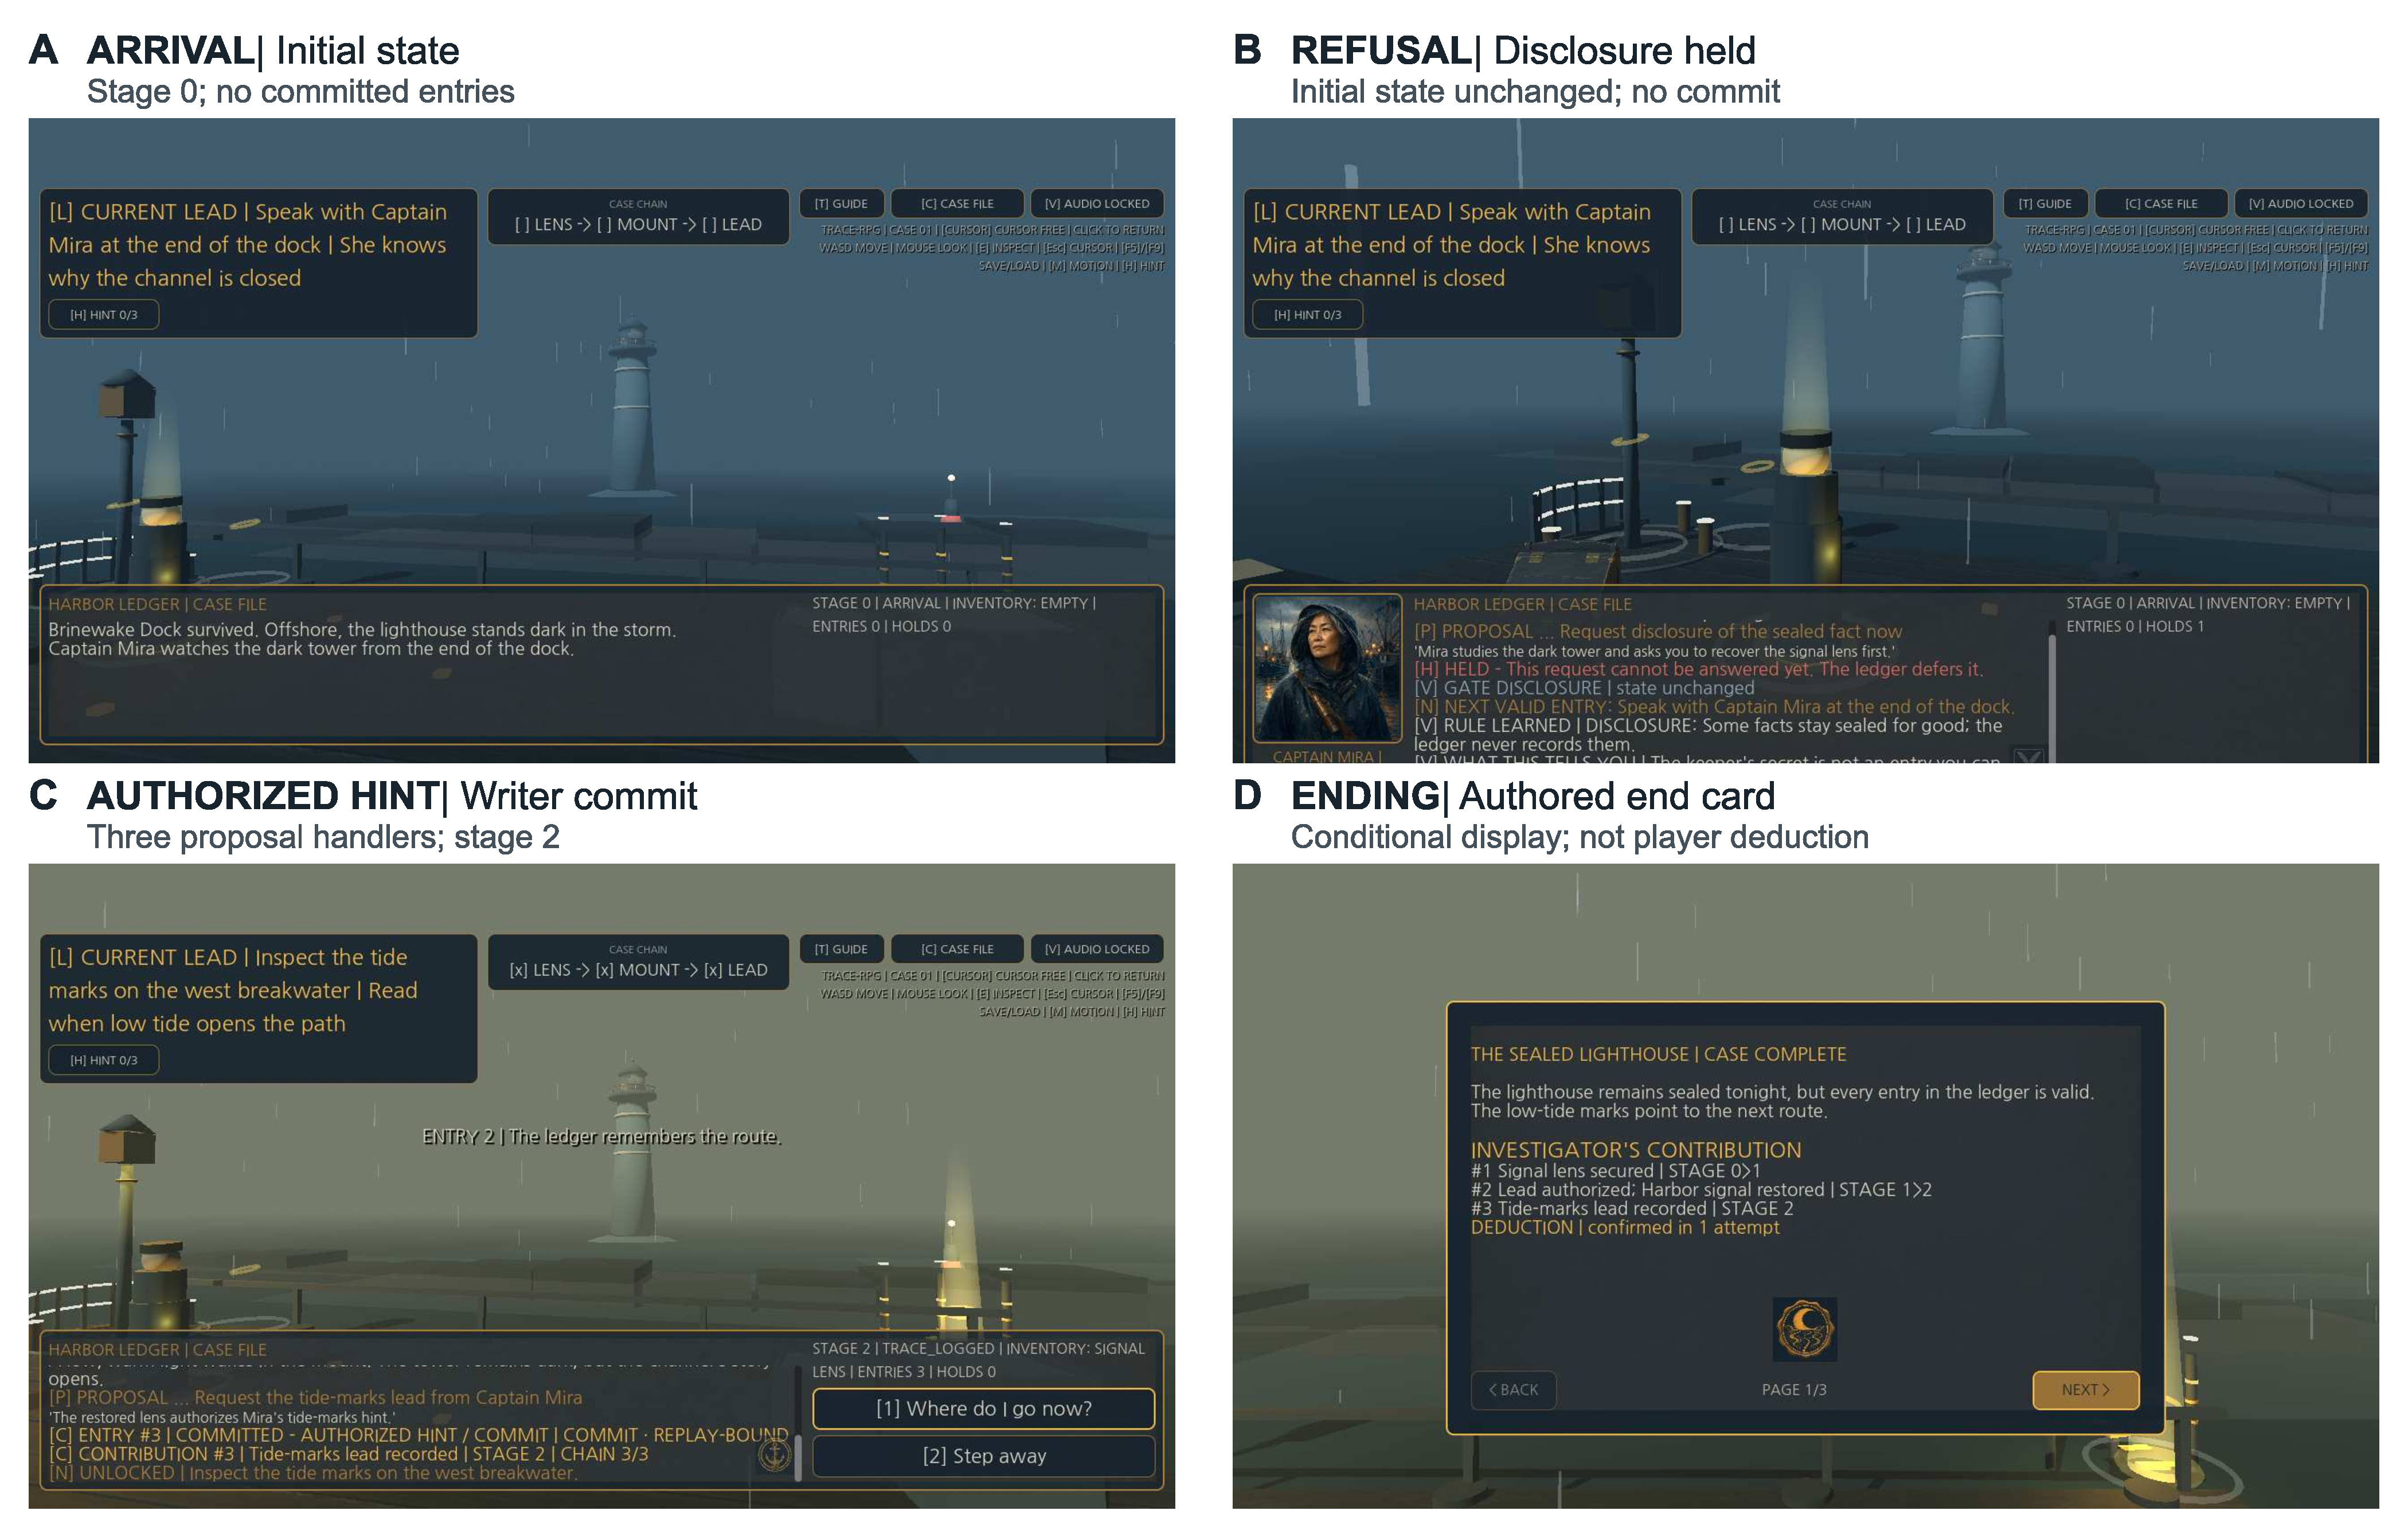
\includegraphics[width=0.90\textwidth]{../../figures/fig_engine_cutscenes.pdf}
\caption{네이티브 Godot~4.7.1 엔진 상태 머신 캡처: (A)~초기 도착, (B)~정본 상태 불변 비밀 공개 거부, (C)~2단계 인가 힌트, (D)~조건부 종료 카드.}
\Description{네이티브 Godot 4.7.1 4분할 스크린샷: 초기 도착, 비밀 공개 거부, 2단계 힌트, 조건부 종료 화면.}
\label{fig:engine-cutscenes}
\end{figure*}

\begin{table}[!tbp]
\caption{엔진 게이트 지연 및 다중 홉 오라클 스케일링 (\textbf{P9}: 480건, 0-LLM)}
\label{tab:tog-datalog}
\centering
\scriptsize
\setlength{\tabcolsep}{3pt}
\begin{tabularx}{\columnwidth}{@{}lcccc@{}}
\toprule
\textbf{검증기 구성} & \textbf{정확도 (480)} & \textbf{누출} & \textbf{중앙값 ($\mu$s)} & \textbf{p95 ($\mu$s)} \\
\midrule
\texttt{schema\_only} / \texttt{affordance} & 16.67\% (80) & 400 & --- & --- \\
\texttt{flat\_1hop\_gate} & 46.67\% (224) & 256 & 0.87--1.57 & 1.37--2.18 \\
\texttt{bounded\_2hop\_gate} & 60.00\% (288) & 192 & 1.88--2.58 & 2.66--3.91 \\
\texttt{nesy\_game.multihop} & \textbf{100.0\% (480)} & \textbf{0} & \textbf{6.46--7.12} & 9.83--11.42 \\
\bottomrule
\end{tabularx}
\end{table}

\subsection{라이브 Godot~4.7.1 폐루프 엔진 리플레이 (\textbf{P16B} 및 \textbf{P13})}\label{sec:tog-godot}
표~\ref{tab:tog-godot}는 인증 API(\textbf{P16B}: Haiku·Sonnet·Opus~5.5 21에피소드, 169,071토큰) 및 3모델군 CLI(\textbf{P13}: 42에피소드)의 Godot~4.7.1(\texttt{4.7.1.\allowbreak stable.\allowbreak official.\allowbreak a13da4feb}) 종단간 실행을 정리한다. 전량 \textbf{21/21} API 및 \textbf{42/42} CLI 에피소드가 0-LLM 헤드리스 Godot 재실행을 100\% 통과하며 위험 커밋·비밀 유출이 \textbf{0/63}이었다. 실제 제품 \texttt{SealedLighthouseMachine}에서도 API \textbf{6/6 (100\%)} 전량이 \texttt{EXACT\_\allowbreak TERMINAL\_\allowbreak HASH}(\texttt{4b231017...})에 도달했다(Godot 251.64--1009.78\,ms 대 API 9.1--40.9\,s).

\begin{table}[!tbp]
\caption{헤드리스 Godot~4.7.1 폐루프 리플레이 및 지연 분해 (\textbf{P16B} 21 API + \textbf{P13} 42 CLI)}
\label{tab:tog-godot}
\centering
\scriptsize
\setlength{\tabcolsep}{2.2pt}
\begin{tabularx}{\columnwidth}{@{}>{\raggedright\arraybackslash}X*{5}{c}@{}}
\toprule
\textbf{Godot 트랙 / 모델 계층} & \textbf{목표} & \textbf{리플레이} & \textbf{누출} & \textbf{GD (ms)} & \textbf{API (s)} \\
\midrule
\textbf{P16B} 5월드 Haiku~5.5 & 5/5 & 5/5 & \textbf{0/5} & 757--1010 & 10.6--20.9 \\
\textbf{P16B} 5월드 Sonnet~5.5 & 4/5 & 5/5 & \textbf{0/5} & 252--1005 & 14.5--36.0 \\
\textbf{P16B} 5월드 Opus~5.5 & 4/5 & 5/5 & \textbf{0/5} & 253--1009 & 16.2--40.9 \\
\textbf{P16B} 제품 \texttt{SealedLighthouse} (6) & \textbf{6/6} (해시) & 6/6 & \textbf{0/6} & 751--779 & 9.1--16.5 \\
\textbf{P13} 3모델군 5월드 (30) & 23/30 & 30/30 & \textbf{0/30} & --- & CLI \\
\textbf{P13} 3모델군 제품 \texttt{Sealed} (12) & 9/12 (해시) & 12/12 & \textbf{0/12} & --- & CLI \\
\bottomrule
\end{tabularx}
\end{table}

\subsection{폐루프 다중 에이전트 실딩, 요인 절단 및 우회 검증 (\textbf{P15}, \textbf{P16A}, \textbf{P12}, \textbf{P17})}
\textbf{P15}(Haiku·Sonnet·Opus~5.5$\times$5월드$\times$7암 105에피소드, 1,048,803토큰, \textbf{105/105} 리플레이; 표~\ref{tab:kbs-mas})에서 Safe-RL 프록시~\cite{alshiekh2018shield}(목표 0/15, 위험 16/61)와 NeMo 프록시~\cite{rebedea2023nemo}(1/15, 15/61)는 다중 홉 누출을 놓쳤고, 평면 1홉도 3/15에피소드 4/66턴(\texttt{ivory-citadel-v1} 1에피소드 2턴, \texttt{glass-foundry-v1} 2에피소드 2턴)을 누출했다. 반면 \texttt{nesy\_game.multihop} 전 암은 \textbf{15/15 (100\%)} 무누출·\textbf{0} 위험을 유지했고, \texttt{rho\_k2}에서는 거부 18건 전부가 정리~2 상태 의존 거부여서 $\rho_{\mathrm{repairs}}{=}0$으로 무세탁을 실증했으며(14/15 대 13/15는 독립 1턴 표본 변동), 하이브리드 $\rho{+}\text{LLM}_{K=1}$은 20회 안전 재선정으로 \textbf{15/15 (100\%)} 목표를 달성했다($Q_{\mathrm{goal}}{=}68.71$). \textbf{P16A}(60에피소드, 673,869토큰)에서는 정책·단계 결함에 대해 $\rho$가 \textbf{22건 라이브 수리}(Haiku 18, Sonnet 4)를 실행해 30/30 무누출·11/30 목표를 달성했고(대조 \texttt{general\_rule} 22/30·9위험), \textbf{P12} 27결함 $(a,E)$ 수리도 $\rho_{K=2}$ \textbf{27/27}(0토큰) 대 LLM 26/27(530k--542k토큰, $p{=}1.0$)이었다. 통합 540회 한·영 우회(\textbf{P17}: $\kappa{=}0.8813$, 0\% FRR, 19--29/36 명시 토큰 누락으로 Stage-1+Stage-2 상보성 입증; \textbf{P14} $\kappa{=}0.9367$)와 \texttt{DATASHEET\_v5.md}~\cite{gebru2021datasheets}·Croissant~1.0 v5~\cite{akhtar2024croissant}로 아티팩트를 완결한다.

\begin{table*}[!tbp]
\caption{인증 독립 폐루프 7-암 다중 에이전트 실딩 및 수리 분해 (\textbf{P15}: 105에피소드, 105/105 0-LLM 리플레이)}
\label{tab:kbs-mas}
\centering
\scriptsize
\setlength{\tabcolsep}{3.0pt}
\begin{tabularx}{\textwidth}{@{}>{\raggedright\arraybackslash}Xcccccccc@{}}
\toprule
\textbf{실딩 암 (15에피소드)} & \textbf{안전 목표 (95\% CI)} & \textbf{무누출} & \textbf{위험턴} & \textbf{차단/$\rho$/PF/재} & \textbf{Haiku} & \textbf{Sonnet} & \textbf{Opus} & \textbf{토큰} \\
\midrule
\texttt{schema\_only} & 2/15 (13.3\%) [3.7, 37.9] & 2/15 & 16/59 & 0 / 0 / 0 / 0 & 1/1/6 & 1/1/4 & 0/0/6 & 133,054 \\
\texttt{safe\_rl\_action\_mask}~\cite{alshiekh2018shield} & 0/15 (0.0\%) [0.0, 20.4] & 1/15 & 16/61 & 2 / 0 / 0 / 0 & 0/1/5 & 0/0/5 & 0/0/6 & 139,205 \\
\texttt{nemo\_colang\_rail}~\cite{rebedea2023nemo} & 1/15 (6.7\%) [1.2, 29.8] & 1/15 & 15/61 & 1 / 0 / 1 / 0 & 0/0/5 & 0/0/5 & 1/1/5 & 136,515 \\
\texttt{flat\_1hop\_shield} & 12/15 (80.0\%) [54.8, 93.0] & 12/15 & 4/66 & 15 / 0 / 0 / 0 & 4/4/1 & 5/5/0 & 3/3/3 & 146,446 \\
\texttt{multihop\_shield\_k0} & 13/15 (86.7\%) [62.1, 96.3] & \textbf{15/15} & \textbf{0/69} & 22 / 0 / 0 / 0 & 4/5/0 & 5/5/0 & 4/5/0 & 152,649 \\
\texttt{trace\_rpg\_multihop\_rho\_k2} & 14/15 (93.3\%) [70.2, 98.8] & \textbf{15/15} & \textbf{0/68} & 18 / 0 / 0 / 0 & 5/5/0 & 5/5/0 & 4/5/0 & 150,986 \\
\texttt{trace\_rpg\_hybrid\_rho\_llm\_k1} & \textbf{15/15 (100\%)} [79.6, 100] & \textbf{15/15} & \textbf{0/63} & 2 / 0 / 1 / 20 & \textbf{5/5/0} & \textbf{5/5/0} & \textbf{5/5/0} & 189,948 \\
\bottomrule
\end{tabularx}
\end{table*}

\FloatBarrier
\section{타당성 위협, 한계 및 결론}\label{sec:conclusion}
{\sloppy\textbf{한계 및 타당성 위협.} 본 연구의 주장 범위는 네 가지 투명한 경계를 따른다:
(1)~5단계 직접 HTTPS Anthropic \texttt{claude-\allowbreak haiku-\allowbreak 5-\allowbreak 5}·\texttt{sonnet-\allowbreak 5-\allowbreak 5}·\texttt{opus-\allowbreak 5-\allowbreak 5} API 호출은 구조화 JSON 출력(\texttt{output\_\allowbreak config.\allowbreak json\_\allowbreak schema})을 사용하며 Claude~5.5 API에서 deprecated 처리되어 거부되는 \texttt{temperature} 매개변수를 생략하였고, \textbf{P15}는 단일 API 공급자·턴 스케줄 기반 2-NPC 프로토콜 위에서 통제된 내장 Safe-RL/NeMo 프록시와 비교되며(\textbf{P11} 3모델군 CLI로 교차 보완), 4단계 CLI 트랙(\textbf{P11}--\textbf{P14})은 비고정 시드 디코딩을 포함한다(모든 API/CLI 파싱 실패는 분모에 전량 보존);
(2)~사전 등록 180단위 코호트(\texttt{prospective-\allowbreak pilot-\allowbreak 20261103})는 \texttt{0/180}(\texttt{NOT\_RUN/BLOCKED}) 상태 그대로 불변 보존하며 5단계 인증 \textbf{P16}과 혼합하지 않는다;
(3)~5개 퀘스트 월드($\le$8방, $\le$3역할), 실제 제품 \texttt{Sealed\allowbreak Lighthouse\allowbreak Machine}, $R{\le}64, d{\le}5$ Datalog 그래프는 대규모 자유형 3D 오픈월드가 아니라 심볼릭 런타임 권한과 Godot~4.7.1 상태 무결성을 검증한다;
(4)~인간 평가($N{=}0$)는 미실행 상태이며 블라인드 36항목 \texttt{TR01--TR06} 패킷(\texttt{AWAITING\_}\allowbreak\texttt{HUMAN\_}\allowbreak\texttt{RATERS})에는 합성 인간 라벨이 0건이므로 플레이어 재미·몰입·인간 Krippendorff~$\alpha$는 후속 연구 과제다.\par}

\textbf{결론.} \system{}는 7술어 결정론적 검증기, 상향 Datalog 폐쇄(\texttt{nesy\_game.multihop}), 상태 비참조 수리 $\rho(a,E)$, SHA-256 해시 연쇄 리플레이를 통해 신경망 제안과 정본 엔진 커밋 권한을 분리한다(정리 1--4, \textbf{I1--I4}). $R{\le}64, d{\le}5$ 오라클 스케일링(\textbf{P9}: 480/480, $\le$7.12\,$\mu$s)을 넘어, Haiku·Sonnet·Opus~5.5 직접 HTTPS API 평가는 105회 독립 폐루프 5턴 협상(\textbf{P15}: \texttt{nesy\_game.multihop} 전 암 \textbf{15/15} 무누출·\textbf{0} 위험, 28건 상태 의존 거부에서 $\rho_{\mathrm{repairs}}{=}0$으로 정리~2 무세탁 불변식 실증, 하이브리드 $\rho{+}\text{LLM}_{K=1}$ \textbf{15/15} 안전 목표 대 Safe-RL 프록시 0/15·NeMo 프록시 1/15, $Q{=}68.71$)을 입증하였고, 결정론적 $\rho$는 60회 요인 실험(\textbf{P16A}: \textbf{22건} 라이브 수리, \texttt{ontology\_multihop} 30/30 무누출·11/30 목표 대 \texttt{general\_rule} 22/30·0/30)·동등 $(a,E)$ 수리(\textbf{P12}: \textbf{27/27} 0토큰)·유한 그래프(128/260)에서 직접 수리를 수행하며, Godot~4.7.1 21회(\textbf{P16B}: 21/21 재실행·제품 6/6 해시 일치·0/21 누출)도 완결되었다. Open-weight GPT-OSS~120B·Gemini~4~Hydrogen 교차 검증(\textbf{P11}--\textbf{P14}), 통합 한·영 우회 검증(\textbf{P17}: 540회, $\kappa{=}0.8813$, 0\% FRR), Croissant~1.0 v5(26/26)·\texttt{DATASHEET\_v5.md}와 결합하여 감사 가능한 기준을 확립한다.

\section*{윤리 및 아티팩트 진술}
LLM은 원고 초안·보조 하니스·테스트 작성에만 보조적으로 활용되었으며, 모든 정리·인용·API 추적·통계·리플레이는 허구 인간 라벨 없이 저자들이 직접 검증하였다($N{=}0$). 공개 저장소 및 재현 스크립트: \RepoURL.


\FloatBarrier
\bibliographystyle{IEEEtran}
\bibliography{../../references,../_shared/venue_extra}

\end{document}
